\chapter{Implementation of Applications}
Store the current order of product and its meta information, find which shelf stores the current requested product, assign an idling logistic unit to pick up the itinerary ... I/O intensive operations make up the majority of SAP business scenarios. 
 In the load test conducted in this paper, applications are built to realize such a scenario: advertisements are published in a bulletin board and clients can browse through the items. 

The PostgreSQL backing service from Cloud Foundry is used as the database. As the goal is to test how the application handles large amount of concurrency instead of the database efficiency, data will not be queried in high quantity or by complicated SQL actions in the test. 

\section{Implementation Configuration}
To bring Java and Node.js to a comparable level, the applications are implemented with minimum use of frameworks so that the overhead or any other influential factors on performance can be first taken off the table.

 \begin{figure}[h]
 	\centering
 	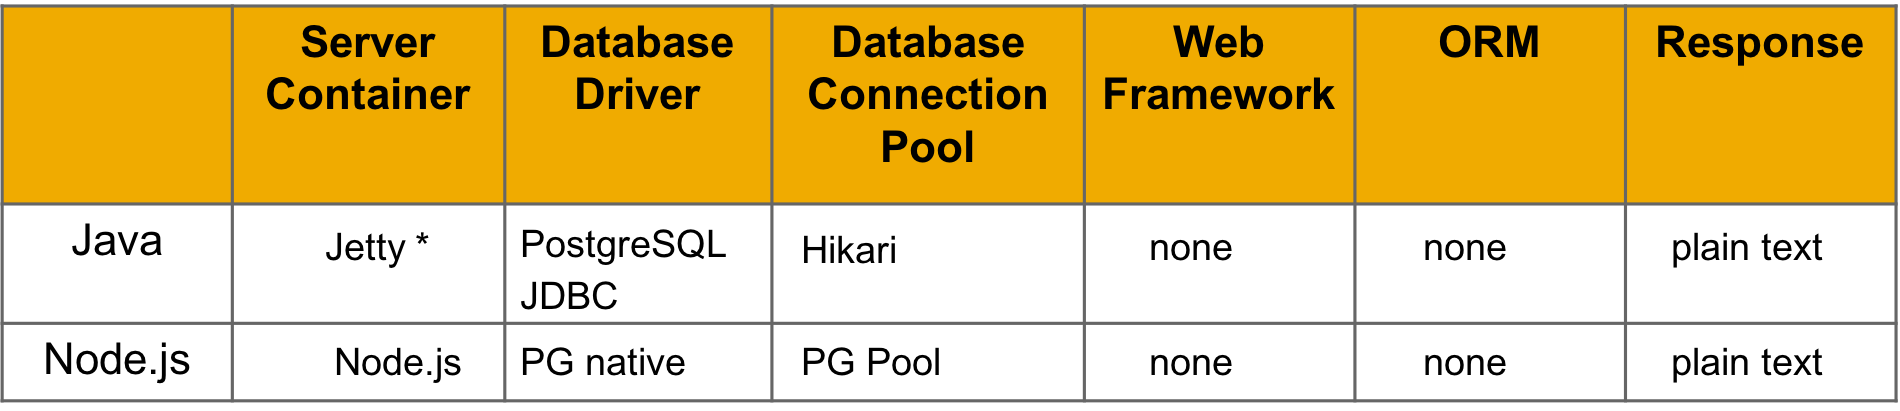
\includegraphics[width=12cm]{implementation}
 	\caption{Implementation configuration}
 	\label{implementation}
 \end{figure}

As table \ref{implementation} shows,  the implementation of both applications utilize no REST or any other kind of web framework. No ORM is applied. Response is sent as plain text to the client to avoid overhead brought by using framework to do JSON serialization/deserialization. \\
Java application uses embedded Jetty server to handle plain HTTP requests because its lightweight. (* There is an even simpler built-in HTTP server from Oracle JRE. However, the build pack used in Cloud Foundry is OpenJDK JRE.)  Node.js application uses its embedded web platform. The connection with database is plain JDBC for Java while Node.js uses a popular PostgreSQL library: PG. Since the data structure is intentionally kept simple: only one table and with no complex data types, the application without ORM doesn't bring about a lot of boiler plate code.  \\

\section{optimize the Java implementation}
All possible attempts are made to bring about every potential performance of the application. Since there is no complex logic, the focus of optimization lays on the interaction between applications and database. In case of Java implementations, to set a optimal thread pool configuration is also investigated. \\
The first checkpoint is database connection which greatly affect performance since it is the most expensive operation in the application without a complicated computing logic. Opening a connection and closing it with every request would gigantically slow down the application. Therefore connection pool is a key component in the implementation. It turns out there are quite a few libraries which handles connection pooling. In the thesis,  three different libraries are tried out. \textit{PGPoolingDataSource}  \citep{pgpool}   comes with default PostgreSQL JDBC driver. \textit{commons-dbcp2} \citep{dbcp} is from Apache Software Foundation. \textit{HikariCP} is a "zero-overhead" production ready connection pool. It turns out \textit{HikariCP} \citep{hikari} has outperformed the other two. \\
The next thing is to find an ideal configuration for the connection pool size. In an article from Brett Wooldridge \citep{poolsize}, it is pointed out larger connection pool size configuration doesn't necessarily lead to a better performance. Single core can only execute one thread at a time; then the OS switches contexts and that core executes code for another thread, and so on. Given a single CPU resource, executing A and B sequentially will always be faster than executing A and B "simultaneously" through time-slicing. Theoretically, the database will be slowed down the moment connection pool size exceeds the total core number. However, there are a few other factors at play. For example, databases typically store data on a disk, which traditionally is comprised of spinning plates of metal with read/write heads mounted on a stepper-motor driven arm. So there is a time cost for disk "I/O wait". During this time the OS could put that CPU resource to better use by executing some more code for another thread. Because threads become blocked on I/O,  more work can be done by having a number of connections/threads that is greater than the number of physical computing cores.
\begin{figure}[h]
	\centering
	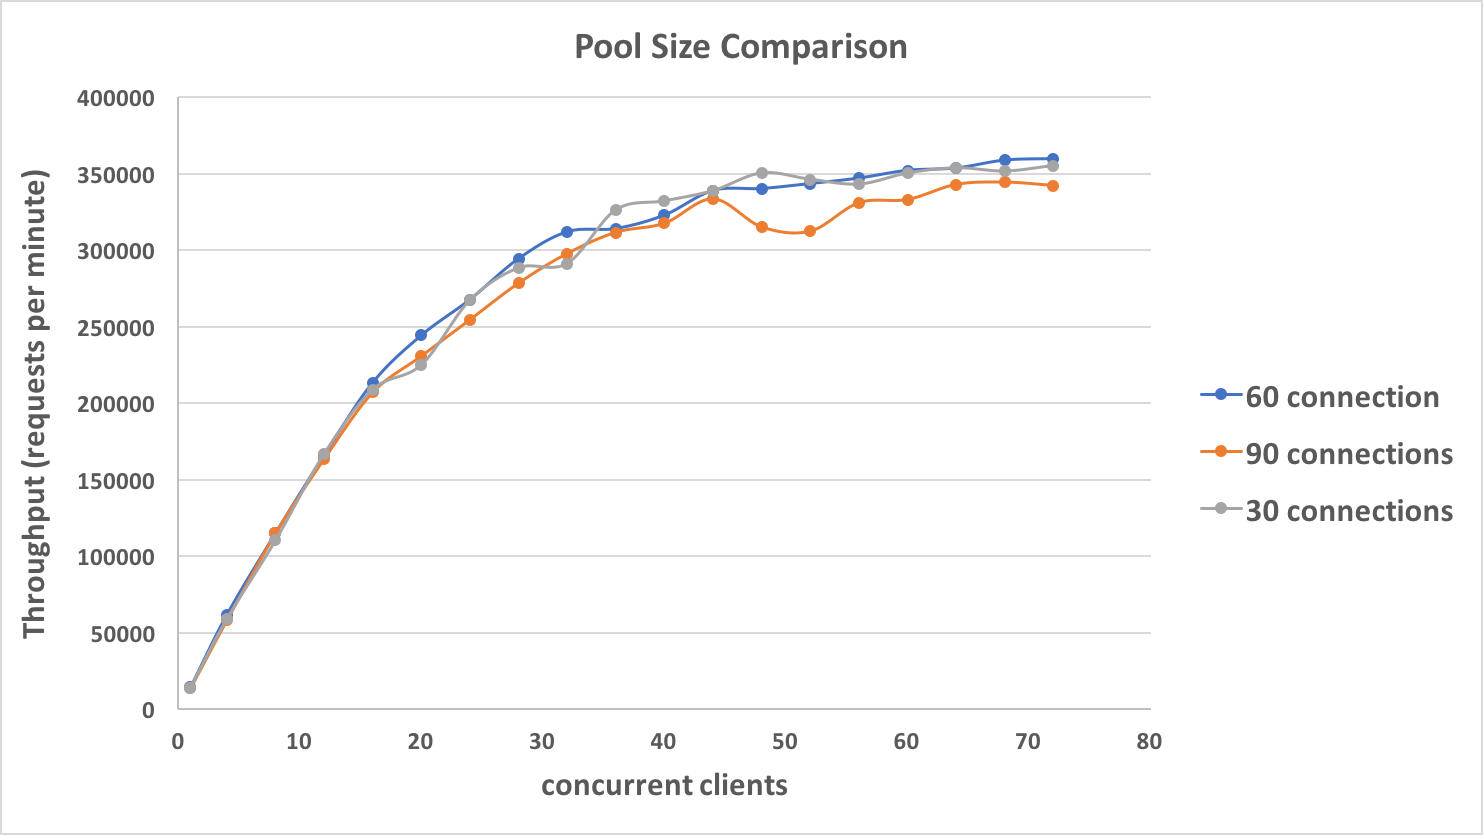
\includegraphics[width=12cm]{pool_size_con_user}
	\caption{Database connection pool size comparison}
	\label{pool-comparison}
\end{figure}
In the case of thesis, database is running in Diego cell which contains 4 CPUs. In order to verify and find the best fit for the load the thesis intend to generate, an experiment is conducted with connection pool size of 30, 60, and 90.  Figure \ref{pool-comparison} shows a slight difference can be deducted that the pool size of 90 reaches the upper limit of total transaction slightly earlier than the other configurations. A little bit better is the performance from a connection pool size of 60 than that of 30. Then we compared the end-to-end response time with the data base response time.  As figure \ref{ete-vs-db} shows, when the response time peaks, the database response time stays stable and can hardly be considered responsible for the peak. Since the database pool size doesn't pose a conspicuous difference, we can draw the conclusion that the database is working at a high speed with no noticeable delay. The pool size setting is not a deciding bottleneck at all. It could be because the database is a docker container version and has no dedicated virtual machine. Thus it lies likely quite near the application and has little network overhead. 

\begin{figure}[h]
	\centering
	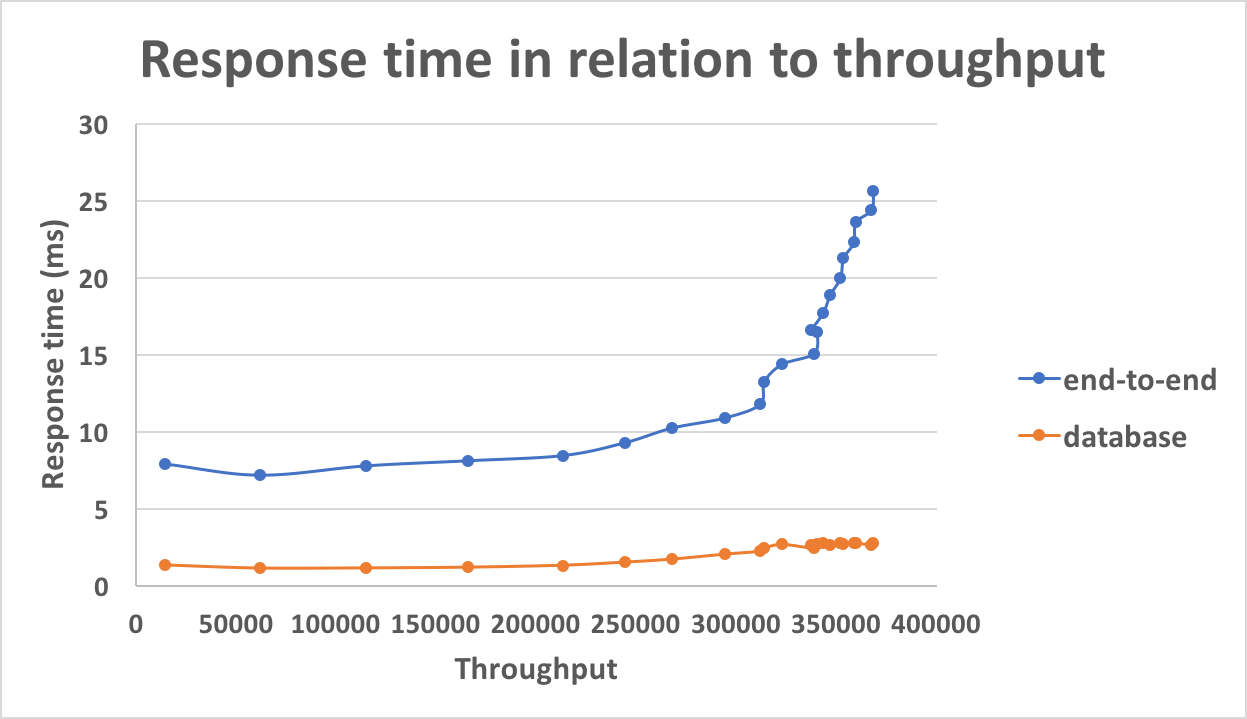
\includegraphics[width=12cm]{ete-vs-db}
	\caption{Comparing end-to-end response time with database response time}
	\label{ete-vs-db}
\end{figure}

Thread pool size is also scrutinized for Java application and following the recommendation made by Jetty \citep{threadpool}, the size is set from 10 to 400. \\


\section{Optimize the Node.js implementation}
Node.js application basically faces the same configuration of connection pool in database. In the thesis, also three different libraries are tried out. Unlike Java libraries, there is some overlapping with regard to the Node.js libraries. In npm, one can find a number of PostgreSQL drivers. However, majority of them are built on the basis of one library: "node-postgres/pg" \citep{node-pg}. They are either wrappers or additional implementation with "promise" or "async/wait". For example, a great difference can not be derived from using of "node-postgres/pg" and "pg-promise" in the scenario in this thesis. The comprehensive research on framework benchmarking \citep{Benchmark} uses "Sequelize", which is also tried out in the thesis. However, it yields even a worse performance result because the object mapping costs indisputably computing time. In the end, the suggestion from "node-postgres/pg" writer is adopted to use "pg-native" which can boost a 20-30\% increase in parsing speed.\\




